\documentclass[aps,rmp, twocolumn]{revtex4}
%\documentclass[a4paper,10pt]{scrartcl}
%\documentclass[aps,rmp,twocolumn]{revtex4}

\usepackage[utf8]{inputenc}
\usepackage{amsmath,graphicx}
\usepackage{color}
%\usepackage{cite}

\newcommand{\Richard}[1]{{\color{red}Richard: #1}}
\newcommand{\LH}{\mathcal{L}}
\newcommand{\rvec}{\mathbf{r}}


\begin{document}
\title{On the robustness and consistency of phylogeographic inference}
\author{Richard A.~Neher}
\date{\today}
\begin{abstract}
Continuous phylogeographic inference is a popular method to reconstruct the spatial distribution of ancestral populations and estimate parameters of the dispersal process.
While the underlying probabilistic models can be complex and their parameters are often computationally demanding to infer, these models typically ignore that replication and population growth are tightly coupled to spatial location: populations expand into fertile uninhabited areas and contract in regions with limited resources.
Such coupling, in particular when habitats change over time, can result in biased and overconfident estimates of ancestral locations and dispersal parameters.
These distortions depend in complicated ways on the past dynamics of habitats and underlying population dynamics and dispersal processes such that validity of phylogeographic inferences is hard to assess.
\end{abstract}

\maketitle
As organisms replicate, they also disperse in space, resulting in mixing of the population and exploration of new habitats.
The reconstruction of ancestral locations and past migrations from sampling locations of extant individuals, typically in combination with genome sequence information to infer the phylogeny, is known as phylogeography.
Phylogeographic methods are implemented in popular evolutionary analysis software such as BEAST \citep{lemey_bayesian_2009,lemey_phylogeography_2010}.
The underlying model of dispersal is typically assumed to be diffusive, that is the probability of sampling a descendant at position $\rvec_c$ after time $t$ when the parent was at position $\rvec_p$ is given by
\begin{equation}
    P(\rvec_c| \rvec_p, t) = \frac{1}{4\pi D t}e^{\frac{|r_c - r_p|^2}{4Dt}}
\end{equation}
where $D$ is a diffusion constant with dimensions $\mathrm{length}^2/\mathrm{time}$, and we have assumed a two-dimensional space and ignored anisotropic dispersal.
Such a diffusive process is the simplest and most natural choice in absence of directed motion or long range migration.
It is also mathematically convenient as unknown ancestral locations can be integrated in closed form and the marginal distribution of each position can be calculated exactly for a fixed tree along with the likelihood.
The total likelihood of the configuration is then assumed to be the product of the spatial likelihood and the phylogenetic likelihood, that is the tree topology and branching rates of the tree are assumed to be independent of the spatial process.
This independence assumption is related to the common assumption that all individuals in the population are equally fit.

However, population dynamics is often tightly coupled to spatial location.
Environmental change could mean that a habitat of a population is shifting, resulting in population growth and rapid branching at the expanding edge of the habitat and/or contraction in other areas.
Similarly, invasive species or pathogen might spread into previously areas that support high population densities but where previously empty.
Examples of such shifting habitats are common and range from geological time scales, over decades (climate change), to months (seasonal fluctuations).
In all such cases, the replication process determining the phylogeny of the sample and the spatial location are strongly coupled.

Such coupling can be accommodated in structured coalescent models where the population is divided into discrete subpopulations that exchange migrants and have different population dynamics \citep{vaughan_efficient_2014}.
But the extent to which violations of the independence assumption affect continuous phylogeographic inferences is not well understood.
To accommodate variation not captured by the simple diffusion model, ``relaxed random walk'' models allow the diffusion constant $D$ to vary across the tree (the diffusion constant is integrated over a prior distribution) \citep{dellicour_relax_2021,lemey_phylogeography_2010}.

\begin{figure*}[tb]
    \includegraphics*[width=0.7\textwidth]{figures/illustration_tree.pdf}
    \caption{\label{fig:illustration_tree}{\bf Illustration Yule and Kingman trees and the spatial location of the tips.}
    The total tree length of Yule trees is proportional to the number of tips $n$ and the time to the MRCA is $\log(n)$.
    Kingman trees have a total tree length that is proportional to $\log(n)$ and are characterized by rapid merging close to the present. }
\end{figure*}


In a typically Bayesian phylogeographic inference problem, the input data are typically viral genome sequences as well as their sampling times and sampling locations.
Software like BEAST will then sample the posterior distribution of the phylogenetic tree topology, the sampling times and locations of ancestral nodes in the tree, and model parameters like the diffusion constant $D$ and the evolutionary rate $\mu$.
Results can be estimates of the ancestral location of a particular groups of samples, or summary statistics of the dispersal process.
Popular summaries include empirical estimates of the diffusion constant  \citep{pybus_unifying_2012,trovao_bayesian_2015} and a so-called \emph{dispersal velocity} \citep{dellicour_using_2017}. These are calculated from the estimated displacements along branch $i$ with parent $p_i$ given by $d_i = |\rvec_{p_i} - \rvec_{i}|$ and the elapsed time $\Delta t_i$ as
\begin{equation}
    \label{eq:dispersal_parameters}
    D_w = \frac{\sum_{i\in B}d_i^2}{4\sum_{i\in B} \Delta t_i} \quad \mathrm{and}  \quad v_w = \frac{\sum_{i\in B} d_i}{\sum_{i\in B} \Delta t_i}
\end{equation}
where $B$ is the set of all branches of the tree.
Effectively $D_w$ divides the sum of all observed squared displacements by the total time elapsed on the tree to obtain an estimate of $D$.
It is known as the `weighted' estimate of the diffusion constant.
The weighted dispersal velocity estimate compares the sum of absolute values of observed displacements to the total time, which has dimensions of a velocity.
Alternative formulations use the mean of fractions $D_b = |B|^{-1} \sum_{i\in B}d_i^2/4\Delta t_i$ or $v_b = |B|^{-1} \sum_{i\in B}d_i/\Delta t_i$ instead of the ratio of sums.
We refer to these here as `by branch' estimates.
The latter tend to be dominated by short branches and thus noisier \citep{trovao_bayesian_2015}.

The purpose of this note is to explore how sensitive phylogeographic inferences are to model assumptions and what quantities can be robustly estimated.
My focus here is only on the ability and robustness to estimate dispersal parameters and ancestral locations and I will assume perfect knowledge of the tree and the sampling locations.
So no tree-sampling will be necessary.

\section*{Consistency of summary statistics of dispersal parameters.}

The estimators in Eq.~\ref{eq:dispersal_parameters} are commonly used to summarize dispersal of lineages.
While the estimator $D_w$ directly estimates a parameter of the model and its behavior has been studied in simulations \citep{pybus_unifying_2012}, it is unclear what $v_w$ is measuring and how it behaves.
I simulated diffusion along trees from a Kingman \citep{kingman_coalescent_1982} and Yule \citep{yule_iimathematical_1997} tree ensembles and evaluated the different estimators.
Kingman trees are the classical neutral model of a constant size population, while Yule trees capture features of growing populations (see Fig.~\ref{fig:illustration_tree}).

\begin{figure}[tb]
    \includegraphics*[width=0.48\textwidth]{figures/kingman_dispersal.pdf}
    \caption{\label{fig:D_and_v}{\bf Empirical summary statistics of $D$ and ``dispersal velocity'' for different sample sizes.}
    While diffusion constant $D$ (equal to 1 in this example) can be robustly estimated from simulation data of the underlying model, the dispersal rate $v_w$ (weighted) and $v_b$ (by branch) are not well-defined quantities. Their numerical value depends strongly on sample size and there is no ground truth to compare to. The expected scaling $\sim \sqrt{n}$ of $v$ estimates is indicated by the dashed line.}
\end{figure}


Fig.~\ref{fig:D_and_v} shows empirical estimates of diffusion constants and velocity as defined in Eq.~\ref{eq:dispersal_parameters} from simulated data using freely diffusing locations along Kingman trees.
The diffusion constant $D$ can be estimated robustly from these data and the estimates are compatible with the diffusion constant used to simulate the data $D=1$.
Values of $v_w$ and $v_b$, however, depend strongly on the sample size and are incompatible with each other.
That the velocity estimates are ill-defined is not surprising: By changing the sample size, the average length of branches changes. Diffusion along each branch results in a displacement of $d_i \sim \sqrt{4D\Delta t_i}$ such that a quantity that depends on $d_i / \Delta t_i \sim 1/\Delta t_i^{1/2}$ will change with the time $\Delta t_i$ that elapsed along the branch.
With more samples in the tree, the average branch length decreases, and the velocity estimate increases.
This expected scaling $\sim \sqrt{n}$ is indicated by the dashed line in Fig.~\ref{fig:D_and_v}.
For Yule trees, the average branch length is independent of the number of samples and the velocity estimates are more stable.
But estimates for $v_w$ and $v_b$ are not consistent with each other.

In either case, estimates of $v_w$ or $v_b$ are not meaningful.
The underlying model is diffusive and has no parameters that individually or combined would have dimensions of a velocity.
There is no ground truth to compare the estimates to and $v_w$ and $v_b$ are just descriptive summaries of spatial spread that can not be compared between datasets.


\section*{Effects of density regulation on population structure and dispersal}
Phylogeographic inference typically assumes that the spatial diffusion process is independent of the branching pattern of the tree and ignores coupling between the two.
Such a coupling, however, is expected since growth rates naturally depend on local population density when organisms compete for resources.
It has been known for a long time that ignoring such coupling leads to unrealistically heterogeneous population densities \citep{felsenstein_pain_1975}.
If one simulates a diffusive spatial process in a square of length $L$ with periodic boundary conditions, the population density shows strong fluctuations whenever the diffusion constant $D<L^2/T_c$, where $T_c$ is the coalescent timescale of the population.
This is seen in the examples in Fig.~\ref{fig:illustration_tree} where the population is distributed in patches corresponding to clades in the tree with large uninhabited areas.

For $D<L^2/2T_c$, the time to the most recent common ancestor $T_{MRCA}$ is too small for the population to spread evenly in the habitat.
This heterogeneity increases substantially for even lower $D$, when the population is essentially a cloud of width $\sqrt{4DT_c}\ll L$.
Fig.~\ref{fig:density_reg}A (black line) quantifies this heterogeneity as the standard deviation of population density in two-dimensional bins of different size relative to the expectation in the case of a spatially well-mixed population.


\begin{figure}
    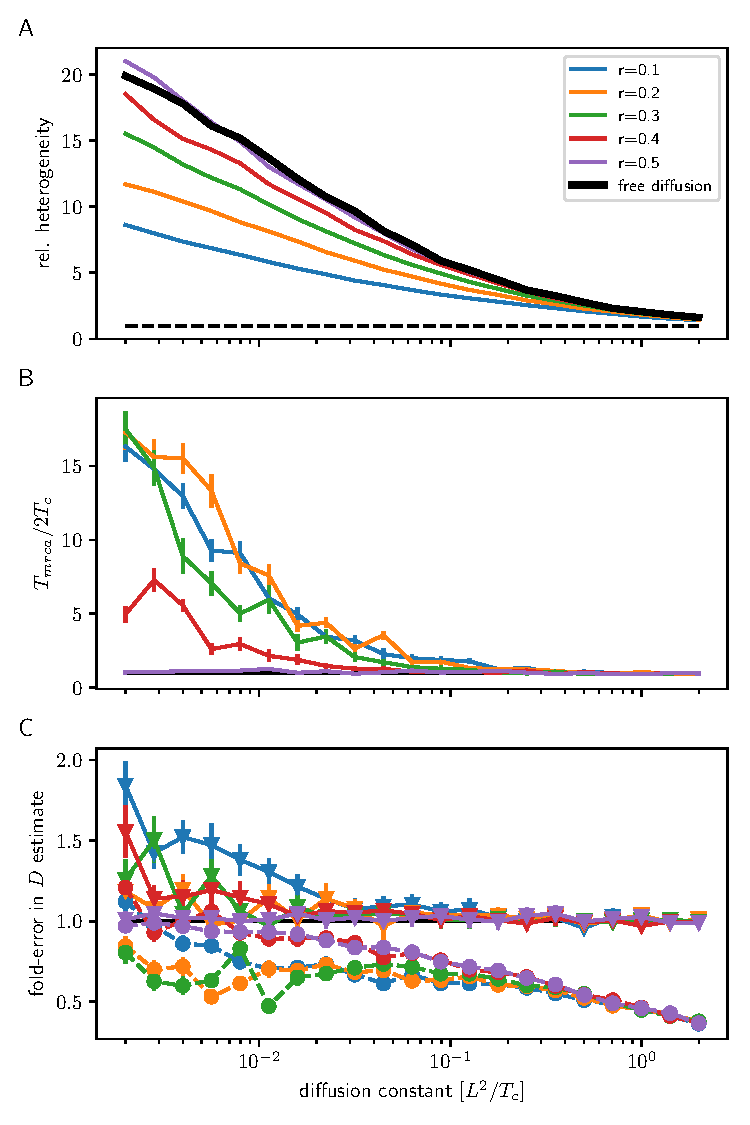
\includegraphics[width=0.53\textwidth]{figures/stable_density}
    \caption{\label{fig:density_reg}  {\bf Effects of population density regulation.}
    When spatial motion is independent of population density and coalescence is sufficiently rapid, the realized population density fluctuates strongly across the habitat. Panel A shows the standard deviation of the population density in bins of linear dimension $L/5$ as a function of the diffusion coefficient relative to the expected value if individuals where independently distributed across the habitat. The thick black line shows the case of free diffusion, the colored lines density regulation with different interaction radii. For $r\ll L$, density fluctuations are strongly suppressed.
    At the same time, the time to the most recent common ancestor increases dramatically (panel B), indicating that the population fragments in subpopulations that don't interact.
    Panel C shows the fold-error of the dispersal estimator $D_w$ for periodic boundary conditions (solid lines, like panels A\&B) and reflecting boundaries (dashed lines).
    }
\end{figure}

Biological populations spread into areas that support them and will quickly populate fertile areas that are below their carrying capacity.
A simple model for the population density $\phi(x,t)$ would be
\begin{equation}
    \label{eq:FKPP}
    \frac{\partial \phi(x,t)}{\partial t} = D\frac{\partial^2 \phi(x,t)}{\partial x^2} + \alpha \phi(x,t)(1-\phi(x,t)/\phi_0)
\end{equation}
where $\phi_0$ is the carrying capacity and $\alpha$ is the population growth rate at zero density.
This model has a stable fixed point at $\phi=\phi_0$.
In a static environment, we thus expect the population density to settle at a constant density $\phi_0$ and density fluctuations will decay with rate $\alpha$.

While dependence of growth (and thus tree structure) on density is a key component of real-world population dynamics, it is difficult to implemented in phylogeographic inference frameworks.
It is, however, fairly straightforward to include density dependence in forward simulations and these simulations can be used to investigate the effect of such coupling between growth and spatial location on phylogeographic inferences.
We calculate the population density using a Gaussian kernel with interaction radius $r$
\begin{equation}
    \phi(\rvec) = \sum_{i\in N} \frac{e^{-|\rvec_i - \rvec|^2/2r^2}}{N\sqrt{2\pi r^2}}
\end{equation}
where the sum is over all individuals $i$ in the population of size $N$.

As soon as the interaction radius $r$ is much smaller than the habitat size, this density regulation leads to a more homogeneous population density, see Fig.~\ref{fig:density_reg}A.
But with decreasing diffusion, the population fragments into smaller and smaller subpopulations that interact only weakly and coalesce slowly.
This manifests in an increasing time to the MRCA, see Fig.~\ref{fig:density_reg}B, which at low $D$ is limited by the time the population was simulated for.
Spatial location and the coalescence process are thus strongly coupled.

Despite the substantial reduction in density fluctuations, the estimates of dispersal rates using Eq.~\ref{eq:dispersal_parameters} are not dramatically affected, see Fig.~\ref{fig:density_reg}C.
If boundary conditions are periodic, that is the habitat has the topology of a torus, estimates $D_w$ of the diffusion constant are accurate for most values of $D$ but slightly inflated when the population is heavily fragmented.
If instead of periodic boundary conditions reflective boundary conditions are used, diffusion constants are underestimated once $\sqrt{2DT_c}$ becomes comparable to the habitat size.
This underestimation of diffusion constants will then result in over-confident inference of ancestral locations, in particular for recent ancestral nodes.

These simulations reveal that both at high and at low diffusion constants, assumptions of phylogeographic inference can be problematic: if diffusion constants are much smaller than then $L^2/T_{mrca}$, the population is fragmented into effective subpopulations and this fragmentation violates the assumptions of phylodynamic models; if $D\gg L^2/T_{mrca}$, the boundaries of the habitat restrict free diffusion, resulting in underestimated dispersal parameters.


\begin{figure*}
    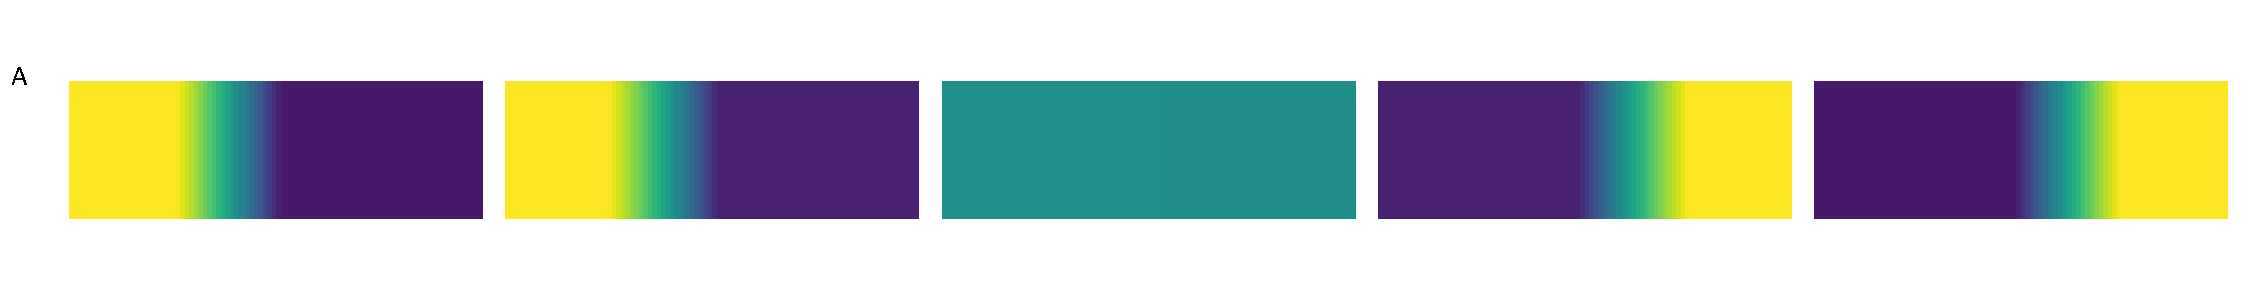
\includegraphics[width=\textwidth]{figures/seasaw_illustration}
    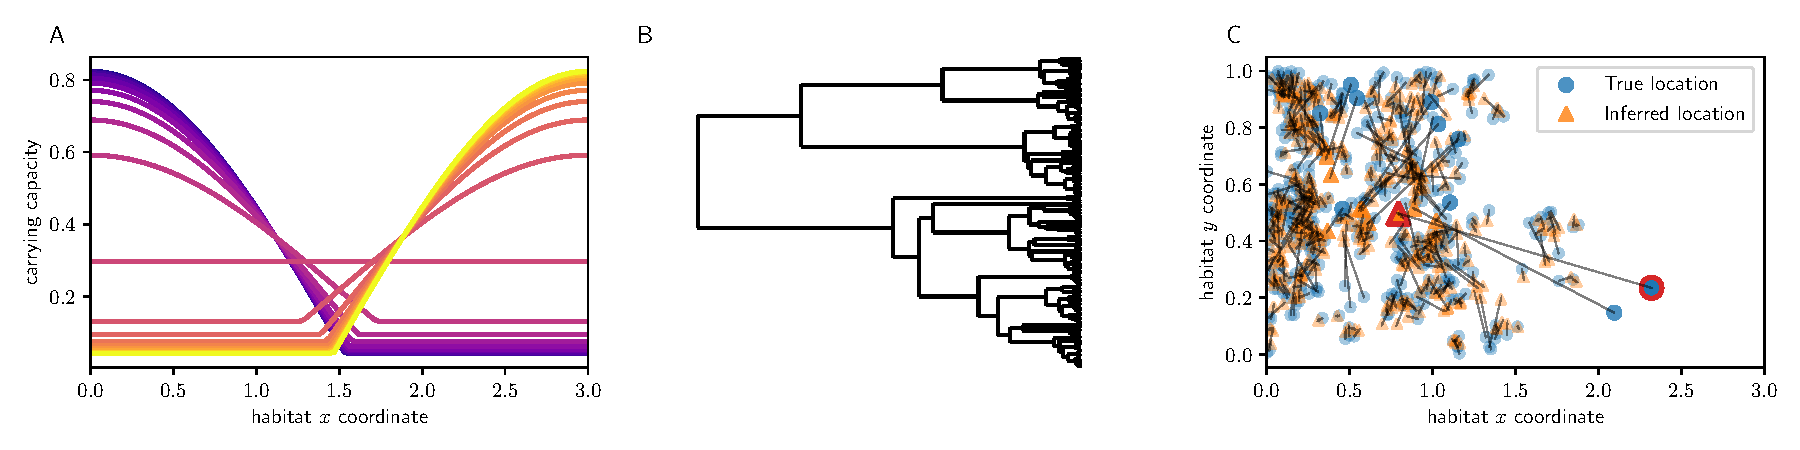
\includegraphics[width=\textwidth]{figures/seasaw_example}
    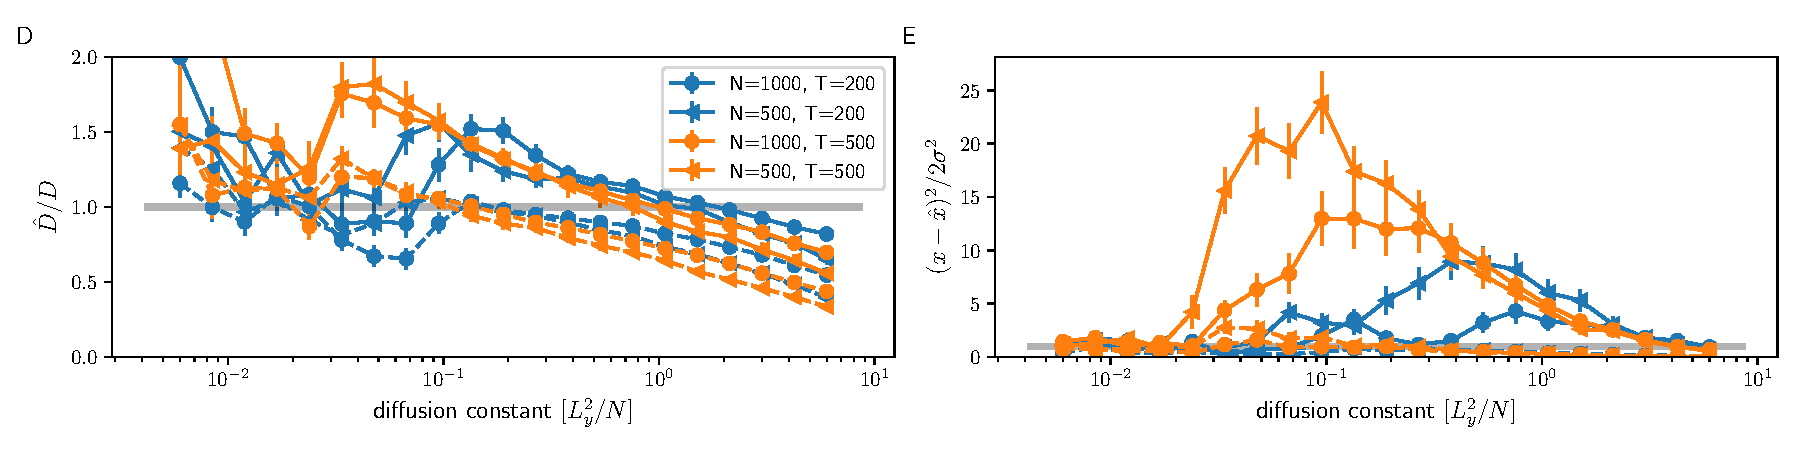
\includegraphics[width=\textwidth]{figures/seasaw}
    \caption{\label{fig:seasaw} {\bf Phylogeographic estimates in rapidly changing environments.} Panel A shows an illustration of the simulated set-up: The carrying capacity first peaks on the left, becomes flat, and then peaks on the right before shifting back. The habitat size is $L_x=3$, $L_y=1$.
    Panel B shows a tree from a simulation under these conditions with $D=0.0008$ and $N=500$, while panel C right shows the inferred (triangles) and true positions (circles) of internal nodes, highlight the root with large markers. Blue and green colors correspond to older nodes, yellow to recent nodes.
    Panels D show estimates of diffusion coefficients in directions $x$ (solid lines) and $y$ (dashed lines) relative to their true values as a function of the true value of $D$. Panel E shows the average $z_x^2$ and $z_y^2$ for the oldest 20\% of internal nodes. Inference of the x-coordinate of ancestral nodes is drastically overconfident for some values of $D$. }
\end{figure*}

\section*{How do changing habitats affect phylogeographic inferences?}
As discussed above, even a static carrying capacity in an equilibrium population can strongly effect population structure, though this structure has limited effects on estimates of ancestral locations and diffusion coefficients beyond boundary effects.
In reality, carrying capacities vary through time.
Such variation happens on all time scales, ranging from geological timescales over millions of years, environmental changes over millennia to seasonal fluctuations.
The circulation of seasonal influenza viruses, for example, varies by many orders of magnitude between summer and winter in temperate climates.
Fluctuations in carrying capacity mean that populations not just spread because individuals move, but also because populations grow in regions where the population density is below the carrying capacity.
In such situations, the accuracy and interpretation of phylogeographic inferences are unclear.

In Fig.~\ref{fig:seasaw} we consider a case where the region with highest carrying capacity shifts from the left to the right in a periodic manner.
The carrying capacity is illustrated in Fig.~\ref{fig:seasaw}A for 5 time points covering half a period.
In between the two extreme left/right concentration of the carrying capacity, carrying capacity is uniform.
To avoid extinction at low dispersal rates, selection is soft, meaning that the overall population size is kept approximately constant even if the entire population is stuck in the unfavorable region.
If the dispersal rate is sufficiently high, however, the population follows the shifting carrying capacity and lineages in the tree undergo directed back-and-forth motion.
Inference of ancestral locations in such situations can be misleading as illustrated in Fig.~\ref{fig:seasaw}B.
The population was sampled at a time when it has just contracted to the left and the positions of older nodes is not estimated correctly.
Their true locations are to the right of the current population, but the inferred location are central in the shifted population.

The severity of such biases depends on the period at which the carrying capacity oscillates and on the dispersal rate, see  Fig.~\ref{fig:seasaw}C.
Fig.~\ref{fig:seasaw}D shows the estimated diffusion constant (using Eq.~\ref{eq:dispersal_parameters}) in $x$ (solid lines) and $y$ (dashed) direction relative to the true value used in the simulations.
At very high diffusion constants, both $D_x$ and $D_y$ are underestimated due to spatial constraint of carrying capacity as also discussed above (see Fig.~\ref{fig:density_reg}).
With decreasing $D$, $D_x$ starts to be overestimated and peaks at a value that depends on the period $T$, before decreasing to (noisy) estimates that are broadly compatible with the true value.
In this range of dispersal rates, the population can no longer follow the shifting carrying capacity.
This decoupling happens at lower values of $D$ for longer periods of environmental change.
With the parameters used in the simulation, the estimates of $D_x$ deviate by a factor of 2 from its true value, which is not dramatic compared to the variation of dispersal rates in nature.

However, along with problematic inference of diffusion coefficients, estimates of ancestral locations are over-confident.
Panel Fig.~\ref{fig:seasaw}E shows $z_x^2 = \langle (\hat{x} - x)^2/\sigma_x^2 \rangle$ and $z_y^2=\langle (\hat{y} - y)^2/\sigma_y^2\rangle$ for the oldest 20\% of internal nodes, where $\hat{x}$ and $\sigma_x$ are the mean and standard deviation of the posterior of $x$, respectively (and analogously for $y$).
If the model estimated ancestral locations consistently, $z_x^2$ should be 1 on average.
Instead, it is as high as 20 for the simulations shown and this over-confident and biased estimations depend in non-monotonic ways on the true diffusion constant and the period of environmental change.
With decreasing $D$, $z_x^2$ increases largely because the expected uncertainty decreases, before peaking when the population can no longer follow the shifting carrying capacity.
A peak value of 10-20 indicates that the typical ancestral location of the deep nodes is 2-4 standard deviations away from the true location, an example of which is shown in Fig.~\ref{fig:seasaw}C.
Conversely, at high dispersal rates, the average $z_x^2$ and $z_y$ are both smaller than one since the estimated uncertainty is larger than the true uncertainty since the diffusion is constrained by the boundaries of the habitat.


The above results show that behavior of a population in shifting habitats and the interpretation of phylogeographic inferences depend strongly on the rate of environmental change and the dispersal rate.
If the population can not follow shifting habitat, the situation is similar to the static case often leads to fragmented populations.
Once the population starts following, inferred ancestral locations of deep nodes become unreliable, while at high dispersal rates expected uncertainties are larger than the habitat size and there is little information on deep ancestral locations.

To study the interplay of moving habitats and phylogeographic inference more systematically, I will now consider a situation where the population is constrained to a stripe with a Gaussian profile that moves at a constant velocity $v$ along the $x$-axis (Fig.~\ref{fig:traveling_wave}).
The dispersal rates necessary to keep up with the shifting carrying capacity can be estimated from the Fisher-KPP equation (Eq.~\ref{eq:FKPP}) above.
This equation admits solutions with a traveling front, that the population ``invades'' the empty territory with velocity $v_{FKPP} = 2\sqrt{D \alpha}$ \citep{fisher_wave_1937,KPP1937,hallatschek_life_2010}.
Note that the model itself does not have an explicit parameter that has dimensions of a velocity.
The speed at which the population invades space is given as compound of diffusion and accelerated growth in regions of low density and only grows like the square root of diffusion constant.


\begin{figure}
    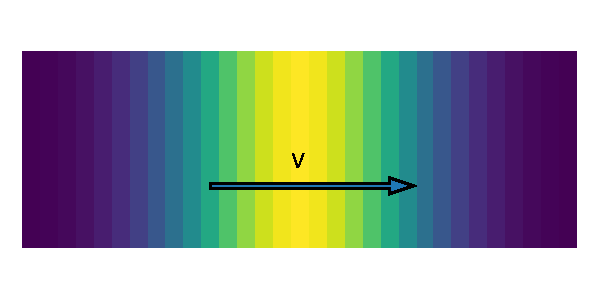
\includegraphics[width=0.3\textwidth]{figures/traveling_wave}
    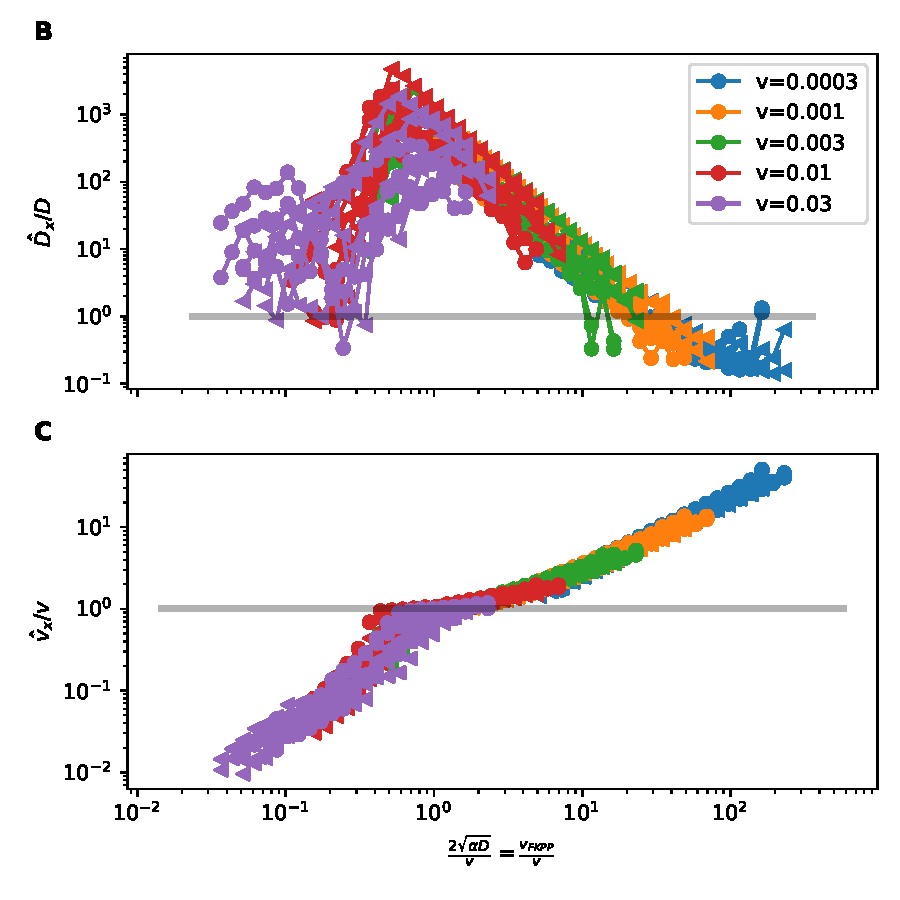
\includegraphics[width=0.48\textwidth]{figures/waves}
    % 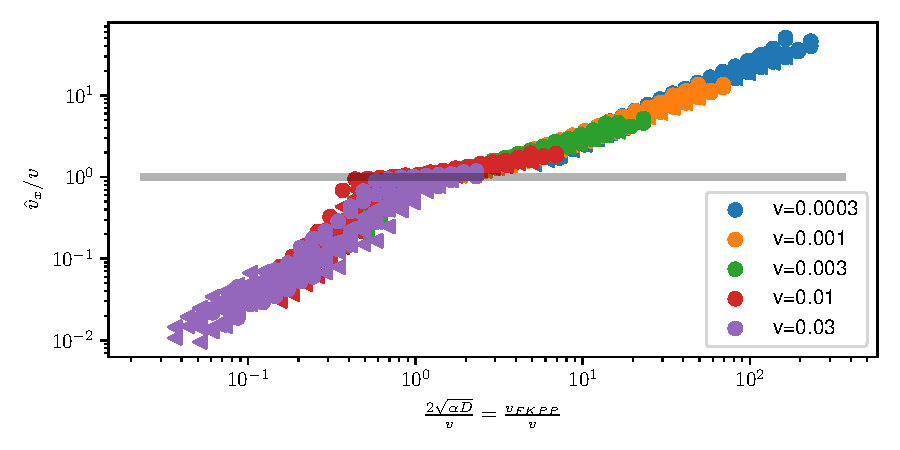
\includegraphics[width=0.48\textwidth]{figures/waves_v}
    \caption{\label{fig:traveling_wave} Panel A shows an illustration of the simulated set-up: a carrying capacity with a Gaussian profile with $\sigma=0.5$ that moves along the $x$-axis with velocity $v$ on a patch with $L_x=3$, $L_y=1$, and periodic boundary conditions.
    Panels B\&C show estimates of diffusion coefficients and velocities, relative to their true values, as a function of the ratio of the FKPP velocity to the external velocity $v$. }
\end{figure}


Fig \ref{fig:traveling_wave}B\&C show simulation results for this traveling habitat. In Panel B, estimates of $D_x$ using Eq.~\ref{eq:dispersal_parameters} are shown as a function of the ratio of the FKPP velocity to the external velocity $v$.
As expected, estimates of $\hat{D}_x$ are often dramatically too high (by up to factors of 1000).
They peak right around when the external velocity matches the FKPP velocity, corresponding to the situation where the population dynamics is maximally affected by the moving carrying capacity.
If the external velocity was lower, undirected dispersal contributes more and more to the displacement of lineages, while the population would be unable to follow the moving carrying capacity if the external velocity was higher.

Fig.~\ref{fig:traveling_wave}C shows estimates of $v$ using Eq.~\ref{eq:dispersal_parameters} relative to the true velocity.
This ratio is monotonically increasing with the diffusion coefficient and shows a range where it close to 1, i.e.~where the estimated velocity of lineages agrees with the external velocity.

These behaviors are explained comparing the speed $v_{FKPP}$ at which the population can invade new territory with the external speed $v$, the ratio of which is used as the $x$-axis in Fig.~\ref{fig:traveling_wave} B\&C.
For $v_{FKPP} \ll v$, the population cannot keep up with the moving carrying capacity and is saved from extinction only because selection is soft.
In this regime, the estimated velocity of lineages is below $v$ and both the estimated $v$ and $D$ increase with $v_{FKPP}$.
Once $v\sim v_{FKPP}$, the estimated lineage velocity coincides with $v_{FKPP}$, while the estimated $D$ peaks at values orders of magnitude above the true value.
For larger $v_{FKPP}$, the estimated velocity is stable for some time, before increasing again with $v_{FKKP}$.
In this latter regime, diffusive motions dominates over directed motion and the estimates of $v$ suffer from the problems shown in Fig.~\ref{fig:D_and_v}.


\section*{Discussion}
Phylogeography aims to reconstruct location and migration of ancestors from the spatial distribution of extant individuals and their genome sequences.
The latter allow the reconstruction of the phylogenetic tree which encodes how closely different individuals are related to each other.
Together with the spatial location of the samples -- the leafs of the tree -- one can reconstruct the likely locations of ancestors and estimate parameters of dispersal.
Popular tools for such inference, however, make strong assumptions about the dispersal process, including assuming that dispersal of individuals is diffusive (i.e.~characterized by small displacements in random directions) and that spatial location is independent of the replication process.
In this note, I have explored the robustness of such inference to violations of the latter assumption while keeping microscopic dispersal strictly diffusive, that is without any long-range migration.

The common practice to estimate dispersal ``velocities'' using displacements of lineages along the tree \citep{dellicour_relax_2021} is problematic.
Firstly, the numerical value of such estimates depends strongly on the sample size and tree ensemble.
Secondly, the underlying model is diffusive and has no parameters that have dimensions of a velocity and even if the quantity could be estimated robustly, there is no interpretation of the quantity within the model.
In cases where a population invades a novel habitat, e.g.~the invasion of North America by the West-Nile virus \citep{pybus_unifying_2012}, the moving front of the population defines a bona fide velocity.
However, as discussed above, this velocity is determined by the interplay of dispersal and population growth at the front.
The velocity is better determined by modeling the position of the front, rather than by tracking individual lineages along the tree.


A more complex set of questions concerns how coupling between growth rate of the population and spatial density affects phylogeographic inferences and how robust these inferences are to shifting habitats.
As has long been known, ignoring the coupling between population growth and spatial location can lead to unrealistic population densities \citep{felsenstein_pain_1975}.
Density regulation leads to homogeneous population densities.
However, the population dynamics strongly depends on whether dispersal is fast enough to explore the entire habitat during the coalescence time $T_c$ of the population in absence of spatial structure.
If $D\ll L^2/T_c$, the population fragments into subpopulations and the time to the most recent common ancestor increases dramatically.
The resulting strong coupling between spatial location and coalescence process violates typical tree priors used in such inference.
In the other case of $D\gg L^2/T_c$, dispersal is rapid enough that ancestral locations of deep nodes are very uncertain compared to the size of the habitat.

Interpretation of such inference becomes even more challenging when habitats shift in time.
Depending on parameters, dispersal rates $D$ can be overestimated or underestimated, sometimes by large factors, and estimates of ancestral locations can be overconfident or too uncertain.
Simulations reveal that this behavior depends on the relative magnitude of the rate at which the habitat shifts and the FKPP velocity which depends on the diffusion constant $D$ and the growth rate in empty regions $\alpha$, as well as curtailed dispersal by the boundaries of the habitat.
The parameter range where both ancestral locations and dispersal parameters are inferred correctly is narrow.

Phylogeographic methods are often studied using West Nile virus and Rabies virus.
West-Nile virus was first detected on the east coast of the US in 1999 and reached the West Coast five years later in 2004 \citep{pybus_unifying_2012}, translating to a wave front velocity of about 1000 km/year.
\citet{pybus_unifying_2012} estimated a diffusion coefficient of between 200 and 5000 km$^2$/day, where the latter refers to branches with particularly high diffusion constant.
Using $v_{FKPP} = 2\sqrt{D\alpha}$ and equating it to 1000 km/year $\approx$ 3km/day, we obtain ranges of $\alpha=\frac{9 km^2}{4 D day^2} = 0.012/day \ldots 0.00045/day$ or between $0.003$ and $0.08$/week.
A pathogen that produces seasonal outbreaks with many orders of magnitude in prevalence between peak and troughs typically requires a growth rate of 1/week, considerably more than what the estimates of $D$ and the FKPP equation imply.
Alternatively, if we assume $\alpha = 0.1/day$, we would expect $D = \frac{10 km^2}{0.4 day} = 25 km^2/day$, implying a daily exploration radius of about 5 km.
This picture is also consistent with the apparent ``slowing down'' of lineages after the initial expansion across North America \citep{dellicour_epidemiological_2020}: Once the habitat was fully explored, directed invasion with $v_{FKPP}$ ceases.
Furthermore, rare long range dispersal could have strongly influenced the spread of the virus in ways not captured by Brownian or relaxed random walks \citep{hallatschek_acceleration_2014}.

Dispersal rates of rabies virus are typically estimated to be between 500 and 1500 km$^2$/year \citep{dellicour_using_2017}.
The most recent common ancestor of various populations is between 30 and 100 years in the past.
This would translate into rather limited spread of 150 to 500km of individual clades from their common ancestor, suggesting that these populations are highly structured (isolated by distance) and that their long range dispersal is dominated by rare introductions of the virus into new populations.

The results presented here and the discussion of the examples above suggested that phylogeographic methods should be used and interpreted with caution.
In many cases the habitat of a population has undergone dramatic and recurrent changes since the $MRCA$ and such changes will affect inferences in ways that are not captured by the models.
In addition, uneven sampling, or complete lack of samples from some regions, can undermine phylogeographic estimates \citep{kalkauskas_sampling_2021,layan_impact_2023}.
The ability to infer ancestral locations is further limited by long-range dispersal \citep{hallatschek_acceleration_2014}.
To capture such deviations from simple diffusive motions, many inference models assume a ``relaxed random walk'', where diffusion constant can vary across the tree according to a broad prior distribution \citep{dellicour_relax_2021}.
However, while such models will often generate a better fit, they don't capture complex interactions between spatial location and population dynamics.

Why does phylogeography then often generate sensible results?
On short time scales, a diffusive model will mostly reduce to a parsimonious reconstruction of ancestral locations which is robust to details of the model.
It is longer time scales, that is deeper nodes in the phylogeny, for which ancestral inferences can get problematic as the chance that the environment has changed and shifted, or that the ancestral locations are in poorly sampled regions, increases.
Inferences, and in particular confidence statements, can be highly unreliable and misleading.
In absence of a good understanding of the dispersal properties and how population dynamics varies and time and space, simple models that allow transparent interpretation of how results are informed by features of the data are preferable to complex and computationally demanding models.


\bibliography{bib}


\end{document}


The above example assumed a habitat that is constant over times comparable to the time to the most recent common ancestor of the population.
If instead the habitat shifts on shorter time scales, the population has to move and such population movement will skew estimates of dispersal.
We simulated such changing habitats by assuming the carrying capacity of the habitat varies periodically in time and space
\begin{equation}
    \phi_0(\rvec, t) = N\left(1 + \sin(2\pi (r_x/L_x + t/T)\cos(2\pi (r_y/L_y + t/2T))) \right)
\end{equation}
This results in moving peaks and troughs in carrying capacity (and thus population density) as illustrated in

\begin{figure}
    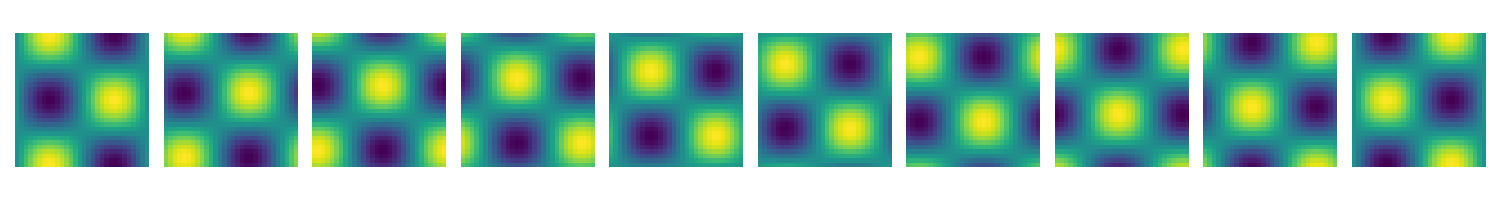
\includegraphics[width=\textwidth]{figures/habitats.png}
    \caption{\label{fig:moving_habitats}}
\end{figure}
